\documentclass[aspectratio=169,10pt]{beamer}
\usepackage{common/pdmtheme}
\graphicspath{{figures/}}
\title[Jetson Orin]{NVIDIA Jetson Orin Nano Super}
\subtitle{A branch that argues against its own hardware}
\author{Predictive Maintenance Platform}
\date{14 October 2026}
\begin{document}

\begin{frame}[plain]
  \vspace{5mm}
  {\LARGE\bfseries NVIDIA Jetson Orin Nano Super}\\[2mm]
  {\large\color{pdmink2} A branch that argues against its own hardware}\par
  \vspace{5mm}\noindent{\color{pdmrule}\rule{\linewidth}{0.4pt}}\par
  \vspace{3mm}
  \begin{columns}[T]
    \begin{column}{0.46\textwidth}
      \scriptsize
      \kv{Compute}{6$\times$ A78AE + 1024-core Ampere}\\[1mm]
      \kv{Rated}{67 TOPS at 25 W}\\[1mm]
      \kv{GPU utilisation}{\textbf{none, by 13\,500$\times$}}\\[1mm]
      \kv{Electricity}{EUR 44/y against the Pi 5's EUR 13}\\[1mm]
      \kv{What survives}{data sovereignty, multimodal fusion}\\[1mm]
      \kv{Cost}{$\sim$EUR 320}
    \end{column}
    \begin{column}{0.46\textwidth}
      \scriptsize\color{pdmink2}
      Two earlier branches already found that accelerators do nothing for
      feature-vector scoring --- Alif on an Ethos-U55, the Pi 5 on a Hailo-8L.
      A third negative result would be a footnote.
      \\[2mm]
      So the brief was inverted: is there a workload here where a GPU is the
      difference between \emph{possible and impossible}, rather than between
      fast and faster?
      \\[2mm]
      \textbf{Never run on a Jetson.} And \texttt{torch} is absent, so the one
      GPU-relevant number is missing --- asserted by a test, not forgotten.
    \end{column}
  \end{columns}
  \srcnote{Branch \texttt{hw/jetson-orin-nano}. 13 tests. Figures from
  \nolinkurl{results/workload_study.json}.}
\end{frame}

% ---------------------------------------------------------------- the study --
\begin{frame}{Three candidates, three negative results}
  \centering
  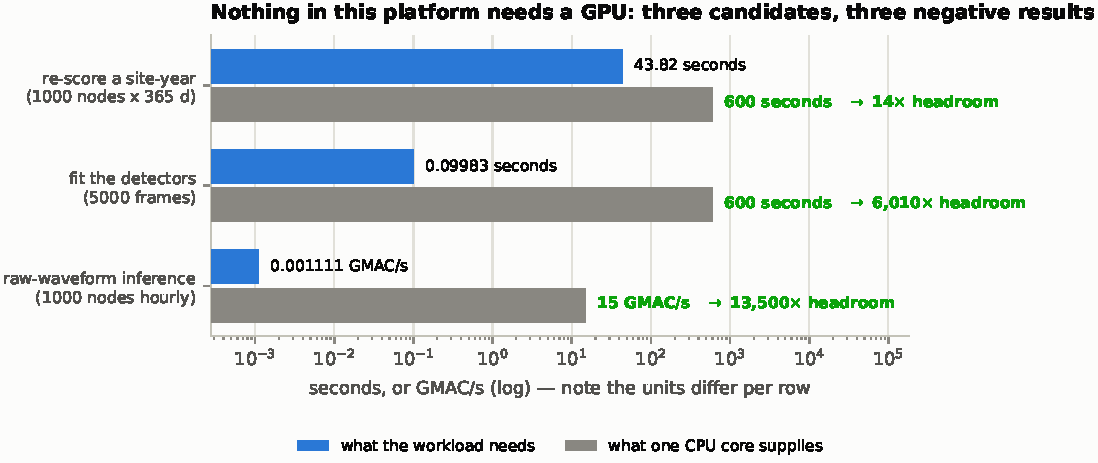
\includegraphics[width=0.80\textwidth]{jetson_headroom.pdf}
  \\[2mm]
  \begin{columns}[T]
    \begin{column}{0.49\textwidth}
      \scriptsize
      Re-scoring a 1000-node site's \emph{entire year} --- 8.76 million frames
      --- takes 44 seconds of CPU. The classical detectors fit in a tenth of a
      second. Raw-waveform inference at hourly cadence is four orders of
      magnitude below one core.
      \\[2mm]
      The study records where candidate 3 would flip:
      \textbf{3\,750 inferences/s}, i.e. 13.5 million nodes at hourly cadence.
    \end{column}
    \begin{column}{0.49\textwidth}
      \scriptsize\color{pdmcrit}
      \textbf{The honest weak spot, and the study says so.}
      \par\color{pdmink2}
      Candidate 2's fits are closed-form and SVD, not gradient descent. A Deep
      SVDD or a 1D CNN is the one training workload a GPU would change,
      \texttt{torch} is not installed here, and so \textbf{that number is absent
      rather than guessed}.
      \\[1mm]
      A test asserts \texttt{torch\_available is False} and fails if torch ever
      appears, so the gap cannot be quietly forgotten.
    \end{column}
  \end{columns}
\end{frame}

% ----------------------------------------------------------- what survives ---
\begin{frame}{What survived: neither justification is about speed}
  \begin{columns}[T]
    \begin{column}{0.49\textwidth}
      \scriptsize
      \textbf{1. Data sovereignty --- implemented.}
      \\[1mm]
      A plant that will not send vibration data off site cannot have its models
      trained in a cloud. Pharmaceutical, defence, and increasingly any site
      whose legal team has read a data-processing agreement.
      \\[1mm]
      That makes the \emph{site} the place where training happens, and a site
      that trains needs more than a gateway. It is the only justification here
      about \emph{where} computation happens rather than how fast --- which is
      why it survives an argument about throughput.
      \\[1mm]
      \texttt{train\_onsite.py} trains from the gateway's own queue, read-only,
      because those frames still have to go upstream.
    \end{column}
    \begin{column}{0.49\textwidth}
      \scriptsize
      \textbf{2. Multimodal fusion --- not written.}
      \\[1mm]
      Vibration + acoustic + motor current + thermal imagery on one asset does
      not fit a 63-float feature vector at all, and the imagery alone rules out
      the MCU and gateway tiers. It is the real GPU case.
      \\[2mm]
      \color{pdmcrit}
      \textbf{Three accelerators in this lineup --- Ethos-U55, Hailo-8L, Ampere
      --- and all three are justified by models that do not exist yet.}
      \par\color{pdmink2}
      That is the honest state of the art here. A stub for any of them would
      make the platform look otherwise.
    \end{column}
  \end{columns}
  \takeaway{Buy it when a legal department makes on-site training mandatory.
  That condition will arrive before the multimodal model does.}
\end{frame}

% --------------------------------------------------------------- the bugs ----
\begin{frame}{Two bugs, both ``checks that cannot fail''}
  \centering
  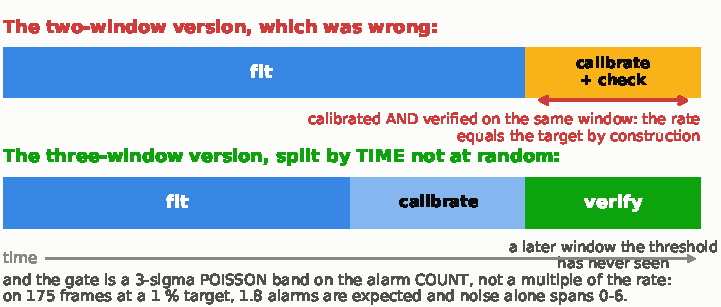
\includegraphics[width=0.84\textwidth]{jetson_gate.pdf}
  \\[2mm]
  \begin{columns}[T]
    \begin{column}{0.49\textwidth}
      \scriptsize
      \textbf{The circular check.} Fit on 75 \%, calibrate the threshold on the
      last 25 \%, then measure the false-alarm rate on \emph{that same} 25 \%.
      \\[1mm]
      That equals the target by construction. The check could never fail, and a
      deliberate 4$\times$ drift sailed through it reporting exactly 0.010 ---
      which is how the bug announced itself: \textbf{a suspiciously exact
      number}.
      \\[1mm]
      Three windows fix it. The same drift now gives 96 alarms where 1.8 were
      expected.
    \end{column}
    \begin{column}{0.49\textwidth}
      \scriptsize
      \textbf{The statistically wrong gate.} The replacement refused if the
      verification \emph{rate} exceeded the target by 4$\times$. On 175 frames
      at 1 \%, the expected count is 1.8 and Poisson noise alone spans 0--6 at
      3$\sigma$ --- so it refused stationary data a third of the time.
      \\[1mm]
      \color{pdmcrit}
      In a plant that means re-running training until it passes, which
      \textbf{selects for whichever window looked quiet}: a biased model,
      reached by a procedure that feels like diligence.
      \par\color{pdmink2}
      Fixed with a 3$\sigma$ Poisson band on the alarm \emph{count}.
    \end{column}
  \end{columns}
  \takeaway{A gate expressed as a ratio of rates is really a gate on a count,
  and at small counts the ratio is the wrong parameterisation --- the same trap
  is open in the alarms/day budget and the n-of-m logic.}
\end{frame}

% ---------------------------------------------------------- what it refuses --
\begin{frame}{The refusals are most of the value}
  \centering
  \scriptsize
  \begin{tabular}{@{}llp{0.52\textwidth}@{}}
    \toprule
    \textbf{Gate} & \textbf{Limit} & \textbf{The failure it prevents} \\
    \midrule
    Minimum frames & 400 &
      A 63-feature covariance estimate needs $\sim$189, and the 50/25/25 split
      gives the fit window half \\
    \textcolor{pdmcrit}{\textbf{Minimum span}} &
      \textcolor{pdmcrit}{\textbf{7 days}} &
      \textcolor{pdmcrit}{\textbf{The one that bites.}} A commissioning engineer
      with a day on site has plenty of frames and nowhere near enough span; a
      detector that has never seen a Monday start-up alarms on the first one \\
    Unscoreable frames & excluded &
      A detector trained on clipped acquisitions learns the artefacts, then
      fails to alarm on the real thing because the real thing is \emph{less}
      extreme \\
    \texttt{SPEED\_UNSTEADY} & excluded &
      Their high-order content is smeared, so training on them teaches the
      detector that smearing is normal \\
    Feature-spec mismatch & excluded &
      Mixing spec versions in one fit mixes two different feature layouts \\
    \bottomrule
  \end{tabular}
  \\[3mm]
  \begin{columns}[T]
    \begin{column}{0.49\textwidth}
      \scriptsize
      \texttt{1 of 3 accepted} on a synthetic site: one good channel, one
      refused for a 0.3-day span, one refused for a population that moved.
    \end{column}
    \begin{column}{0.49\textwidth}
      \scriptsize\color{pdmink2}
      The span gate will be argued about on site, and it should be: seven days
      is a \emph{minimum}, not a target. A monthly duty cycle needs a month.
    \end{column}
  \end{columns}
\end{frame}

% ------------------------------------------------------------------ verdict --
\begin{frame}{Verdict}
  \begin{columns}[T]
    \begin{column}{0.49\textwidth}
      \scriptsize
      \begin{tabular}{@{}lr@{}}
        \toprule
        Workload study, 3 candidates   & all negative \\
        On-site training with gates    & 13 tests \\
        Three-window time split        & \checkmark \\
        Poisson verification gate      & \checkmark \\
        Queue not consumed             & \checkmark \\
        \midrule
        Run on a Jetson                & \textcolor{pdmcrit}{no} \\
        \texttt{torch} installed       & \textcolor{pdmcrit}{no} \\
        GPU used at all                & \textcolor{pdmcrit}{no} \\
        Multimodal fusion              & no model exists \\
        Rollout / rollback             & not written \\
        \bottomrule
      \end{tabular}
      \\[2mm]
      \scriptsize\color{pdmink2}
      \textbf{Legacy Jetson Nano (2019):} end-of-life, last JetPack is 4.6 on
      Ubuntu 18.04. Everything here runs on it in principle; deploying an
      unpatched internet-connected Linux to a plant network is a finding, not a
      trade-off.
    \end{column}
    \begin{column}{0.49\textwidth}
      \scriptsize
      \textbf{The output of this branch is a recommendation against its own
      hardware.}
      \\[2mm]
      Buy the Pi 5. Revisit when a legal department makes on-site training
      mandatory, or when a multimodal model exists that genuinely needs a GPU.
      \\[2mm]
      And keep the training pipeline either way --- the gates, the time split
      and the Poisson band are worth having on whatever box the site ends up
      with.
      \\[2mm]
      \color{pdmink2}
      The EUR 31/year of extra electricity is the cheapest part of being wrong,
      which is exactly why nobody examines it. The study exists so somebody
      does.
    \end{column}
  \end{columns}
\end{frame}

\end{document}
